\newpage
\mysubsection{Transaction}

\ifbook{

  \paragraph{} La plupart des applications en ligne ont généralement comme objectif de réaliser des
  \textbf{transactions}. On mesure d'ailleurs très souvent la performance d'un système au nombre de
  transactions effectuées par minute. La notion de transaction est donc au coeur de bien des aspects
  du \textbf{middleware}.

  \paragraph{} Bien que l'usage du terme \textbf{transaction} soit très répandu, son sens n'est
  forcément aussi clairement maitrisé. Nous allons commencer par étudier sa définition. D'après
  \mylink{http://fr.wikipedia.org/wiki/Transaction\_informatique}{Wikipédia} la définition d'une
  transaction (accédée le 27/12/2011) est la suivante:

  \paragraph{} \textit{En informatique, et particulièrement dans les bases de données, une
  transaction telle qu'une réservation, un achat ou un paiement est mise en oeuvre via une suite
  d'opérations qui font passer la base de données d'un état A - antérieur à la transaction - à un
  état B postérieur et des mécanismes permettent d'obtenir que cette suite soit à la fois atomique,
  cohérente, isolée et durable (ACID):}

  \begin{description}
    \item[atomique] \textit{la suite d'opérations est indivisible, en cas d'échec en cours d'une des
    opérations, la suite d'opérations doit être complètement annulée (rollback) quel que soit le
    nombre d'opérations déjà réussies.}
    \item[cohérente] \textit{le contenu de la base de données à la fin de la transaction doit être
    cohérent sans pour autant que chaque opération durant la transaction donne un contenu cohérent.
    Un contenu final incohérent doit entraîner l'échec et l'annulation de toutes opérations de la
    transaction.}
    \item[isolée] \textit{lorsque deux transactions A et B sont exécutées en même temps, les
    modifications effectuées par A ne sont ni visibles par B, ni modifiables par B tant que la
    transaction A n'est pas terminée et validée (commit).}
    \item[durable] \textit{Une fois validé, l'état de la base de données doit être permanent, et
    aucun incident technique (exemple: crash) ne doit pouvoir engendrer une annulation des
    opérations effectuées durant la transaction.}
  \end{description}

  \begin{figure}[hb]
    \begin{center}
      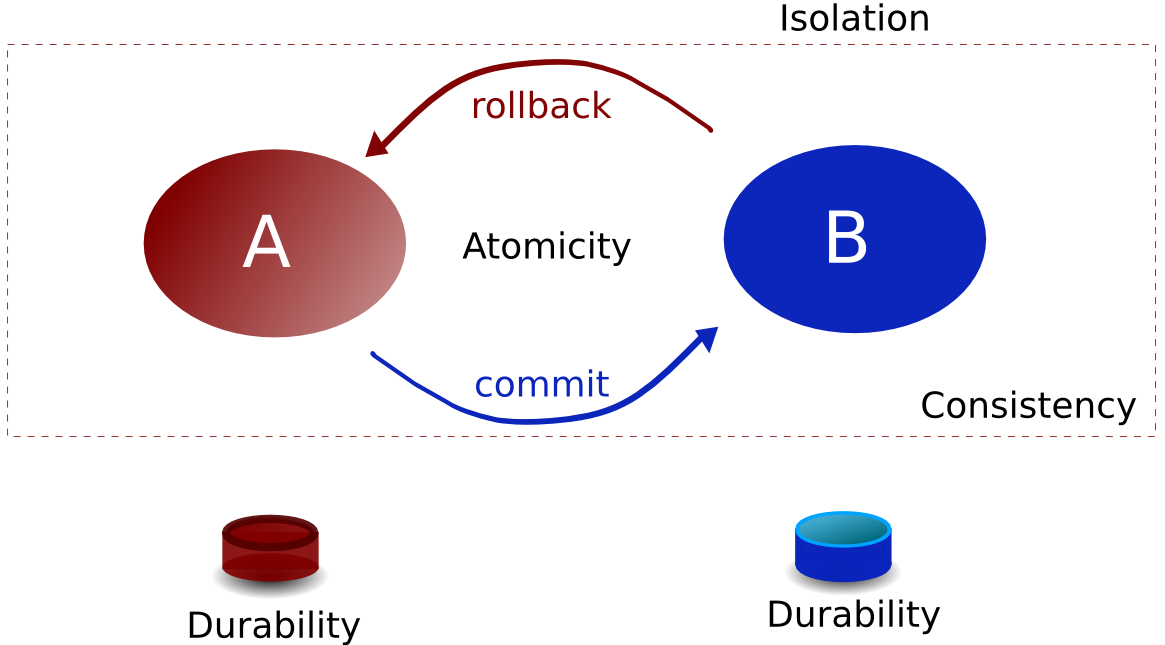
\includegraphics[scale=0.4]{img/transaction.png}
      \caption{Caractéristique d'une transaction}
      \label{tx}
    \end{center}
  \end{figure}
}

\ifslide{
  \begin{frame}{Transaction}
   \begin{center}
     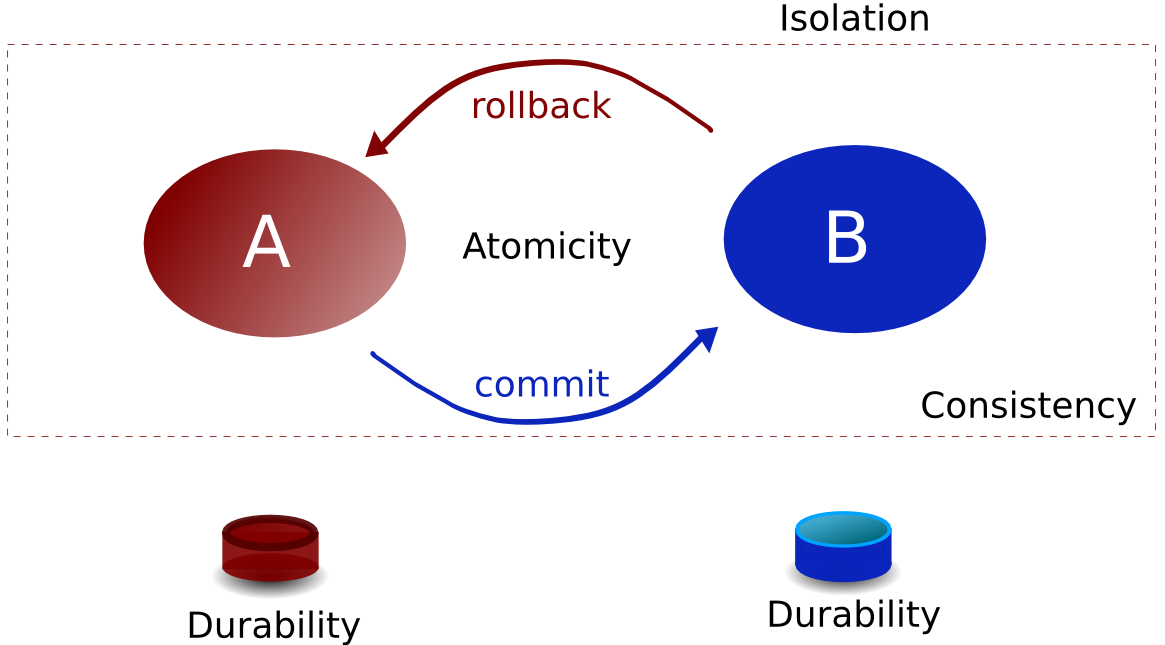
\includegraphics[scale=0.3]{img/transaction.png}
   \end{center}
  \end{frame}
}

\ifbook{

  \paragraph{} L'aspect transactionnel de la plupart des opérations effectuées par un système
  informatique est un point important car c'est souvent à la charge du serveur d'applications ou du
  \textit{middleware} utilisé par l'application de l'assurer.

  \mysubsubsection{Deadlock}

  \paragraph{} Le principal intérêt des transactions réside dans la garantie sur la cohérence des
  données. En effet, l'utilisation de transactions assurent que si deux processus accèdent et
  modifient, de manière concurrente, la même donnée, l'une des opérations n'écrasera pas simplement
  le résultat de l'autre.

  \paragraph{} En effet, la transaction remplit, à ce regard, un peu le même rôle que le système
  d'exploitation dans l'arbitrage des accès aux données entre processus. Prenons un exemple
  simpliciste, pour l'illustrer.

  \paragraph{} Si deux processus cherche à incrémenter une valeur A de manière concurrente,
  hors de toute transaction, le résultat A + 1, puisque lors de leur accès à la valeur, celle ci est
  égale à A, et que les deux requêtes de chaque processus, aboutit à l'enregistrement de la valeur A
  +1. En isolant ces opérations à l'aide de transactions, l'un des processus modifiera la valeur A
  à A + 1, pendant que le second devra attendra la fin de la transaction pour effectuer son
  opération. A l'issu des opérations, la valeur de la donnée est donc A + 2.

  \mysubsubsection{Transaction implicite}

  \paragraph{} Il est aussi important de souligner que même si l'application n'est pas
  transactionnel en tant que tel elle peut utiliser tout à fait utiliser des transactions de manière
  implicite. En effet, de nombreux services ou composant, justement issu du \textit{middleware}
  utilisé par l'application, peuvent tout à fait présenter des aspects transactionnel.

  \paragraph{} Prenons par exemple une application affichant sur un terminal sur un tableau. Elle se
  contente d'effectuer, à intervalles régulier, une opération de sélection sur la table d'une base
  de données et elle n'effectue aucune opération en écriture. En première analyse, il n'y a aucune
  raison pour que l'application soit transactionnel.

  \paragraph{} Elle ne l'est pas, mais elle utilise néanmoins une source de données sur laquelle
  elle effectue des requêtes SQL, qui, elles, sont transactionnelles. Ainsi, pour peu que
  l'application utilise, par ailleurs, un autre \textit{middleware}, lui aussi transactionnel, on
  peut se retrouver face à des problématiques d'isolation ou de \textit{deadlock}, sans que
  l'application métier soit, en tant que tel, transactionnel.

  \mysubsubsection{Coût des transactions}

  \paragraph{} Si effectuer une opération au sein d'une transaction apporte de grande avantage, il
  va s'en dire qu'elle s'accompagne de grandes contraintes et surtout d'un coût certain en terme de
  performance. En effet, sur l'extrait de code suivant, il est aisé d'estimer laquelle des deux
  méthodes est la plus rapide à s'exécuter:

  \begin{figure}[hb]
    \begin{center}
      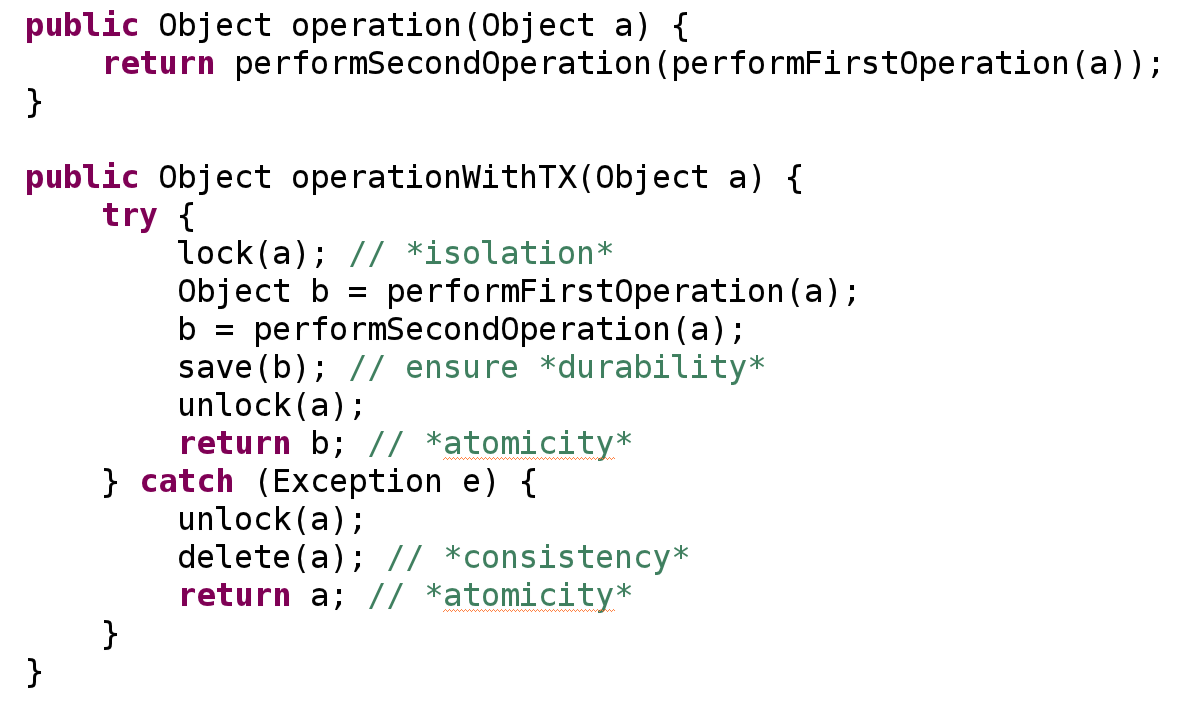
\includegraphics[scale=0.4]{img/transaction-cost.png}
      \caption{Coût en performance d'une transaction}
      \label{tx-cost}
    \end{center}
  \end{figure}

  \paragraph{} Le pseudo code présenté \ref{tx-cost} (page \pageref{tx-cost} n'est fourni
  qu'à titre d'exemple pédagogique. Lors de la mise en place de transaction au sein d'une
  application, le conteneur d'exécution, qu'il s'agisse d'une machine virtuelle ou du serveur
  d'application, fournit une API appropriée.

  % TODO Utilisé l'API et montrer les capacités de monitoring associé ?
}

\ifslide{
  \begin{frame}{Coût en performance d'une transaction}
   \begin{center}
     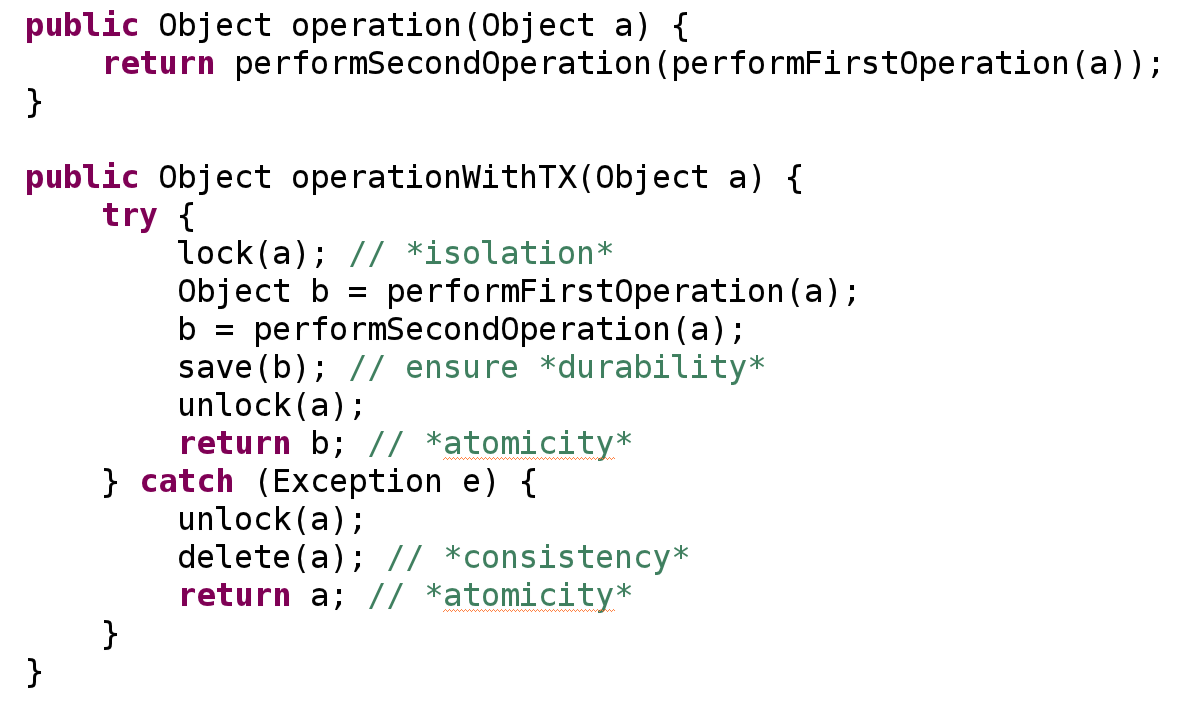
\includegraphics[scale=0.25]{img/transaction-cost.png}
   \end{center}
  \end{frame}
}

\ifbook{
  \mysubsubsection{Être (transactionelle) ou ne pas être (transactionnel) ?}

  \paragraph{} Il est donc bien important, lors de la conception d'une application, de bien
  réflechir à la nécessité ou non d'utiliser des transactions. Une preuve très flagrante de ceci est
  l'émergence des bases de données non transactionnel.

  \paragraph{} Avec l'augmentation des applications "web", mais surtout de leurs nombres
  d'utilisateurs, les bases de données relationnelles deviennent généralement le goulot
  d'étranglement. Comme évoqué précédement, chaque requête vers ces base de données sont en effet
  des transactions exigeant, dans chaque tiers, un certains travail supplémentaire. En supprimant
  l'aspect transactionnel des échanges entres l'applications et la source de données, ces bases de
  données offrent de bien meilleur performance.

  \paragraph{} Bien évidement, on s'expose aussi à des nombreux problèmes de corruption ou pertes de
  données, mais, il existe des applications où ce genre de situation est plus supportable qu'une
  perte de performance.

  \paragraph{} Par exemple, pour un jeu en ligne, que le tableau donnant la liste des 10 dernièrs
  meilleurs scores ne soit pas toujours cohérent et qu'il soit même parfois corrompu n'est pas un
  réel problème. A l'inverse, un le jeu qui devient trop lent, juste parce que les accès au tableau
  des meilleurs scores ralentit l'application, est un réel problème.
}
%- Compensating transaction
